\documentclass[a4paper,12pt]{article}
\usepackage[utf8]{inputenc}
\usepackage{amsmath}
\usepackage{amssymb}
\usepackage{bm} % to get bold epsilon
\usepackage{amssymb}
\usepackage{comment}
\usepackage{graphicx}
\usepackage{xcolor}
\usepackage[left=1.5cm, right=1.5cm, top=2cm, bottom=2cm]{geometry}
\title{\textbf{COM 5120 Communication Theory}}
\author{\textbf{Final Exam Solution}}
\date{December 27, 2022\\
15:30 $\sim$ 17:20
}
\begin{document}
    \maketitle
    \textit{Note}: There are \textbf{6} problems with total 100 points within \textbf{2} pages, please write your answer with detail in the answer sheet.

    {\bf No credit without detail. Closed books. You may use scientific calculator.}

    \begin{enumerate}
     %%%%%%%%%%%%%%%%%%%%%%%%%%%%%%     
        \item (12\%)
            % 1. (Homework #2 - 3, 6.4)
            Let $X$ be a geometrically distributed random variable, i.e., $$P(X = k) = p(1-p)^{k - 1}, k = 1, 2, 3, ...$$
            (a) Find the entropy of $X$. \\ 
            (b) Given that $X > K$, where $K$ is a positive integer, what is the entropy of $X$? \\ \\ 
            \textbf{Solution:} \\
            \textbf{(a)} 
            \begin{align*}
                H(X) &= \ - \sum_{k = 1}^{\infty} p \left(1 - p\right)^{k - 1} \log_2 \left(p\left(1 - p\right)^{k - 1}\right) \\
                     &= \ -p \sum_{k = 1}^{\infty} \left(1 - p\right)^{k - 1} \log_2 p - p \sum_{k = 1}^{\infty} \left(1 - p\right)^{k - 1} \log_2 \left(1 - p\right)^{k - 1} \\ 
                     &= \ -p \log_2 p \sum_{k = 1}^{\infty} \left(1 - p\right)^{k - 1} - p \log_2 (1 - p) \sum_{k = 1}^{\infty} (k - 1)\left(1 - p\right)^{k - 1} \\
                     &= \ -p \log_2 p \cdot \frac{1}{p} - p \log_2 (1 - p) \cdot \frac{1 - p}{p^2} \\ 
                     &= \ - \log_2 p - \frac{1 - p}{p} \log_2 (1 - p) \\ 
                \textbf{[Note]} \;\;\; & \sum_{k = 1}^{\infty} (k - 1)\left(1 - p\right)^{k - 1} = 0 + (1 - p) \cdot 1 + (1 - p)^2 \cdot 2 + \cdots = \sum_{k = 0}^{\infty} k \left(1 - p\right)^{k} \\ 
                                 \text{Let} & \; \sum_{k = 0}^{\infty} k \left(1 - p\right)^{k} = S_n \;\;\; \text{and} \;\;
                                 \left\{ 
                                \begin{aligned}
                                    S_n &= 0 + (1 - p) \cdot 1 + (1 - p)^2 \cdot 2 + \cdots \\
                                    (1 - p)S_n &= 0 + 0 + (1 - p)^2 \cdot 1 + \cdots \\ 
                                \end{aligned}
                                \right. \\ 
                                 % & S_n = 0 + (1 - p) \cdot 1 + (1 - p)^2 \cdot 2 + \cdots \\ 
                                 % & (1 - p)S_n = 0 + 0 + (1 - p)^2 \cdot 1 + \cdots \\ 
                                 \Rightarrow \; & S_n - (1 - p)S_n = 0 + (1 - p) + (1 - p)^2 + \cdots \;\; \Rightarrow \left[ 1 - (1 - p) \right] S_n =  \frac{1 - p}{1 - (1 - p)} \\
                                 \therefore & \; S_n = \sum_{k = 1}^{\infty} (k - 1) \left(1 - p\right)^{k - 1} = \frac{1 - p}{\left[ 1 - (1 - p) \right]^2} = \frac{1 - p}{p^2} \\
                                 & \text{and} \; \sum_{k = 1}^{\infty} \left(1 - p\right)^{k - 1} = 1 + (1 - p) + (1 - p)^2 + \cdots = \frac{1 - p}{p} + 1 = \frac{1}{p}
            \end{align*} 
            \textbf{(b)} 
            Clearly $P(X = k | X > K) = 0$ for $k \leq K$. If $k > K$, then 
            \begin{align*}
                P(X = k | X > K) = \frac{P(X = k, X > K)}{P(X > K)} = \frac{p(1 - p)^{k - 1}}{P(X > K)}
            \end{align*}
            But, 
            \begin{align*}
                P(X > K) &= \ \sum_{k = K + 1}^{\infty} p \left(1 - p\right)^{k - 1} \\
                         &= \ p \left( \sum_{k = 1}^{\infty} \left(1 - p\right)^{k - 1} - \sum_{k = 1}^{K} \left(1 - p\right)^{k - 1} \right) \\
                         &= \ p \left( \frac{1}{1 - (1 - p)} - \frac{1 - (1 - p)^K}{1 - (1 - p)} \right) \\ 
                         &= \ p \cdot \frac{1}{p} - p \cdot \frac{1}{p} - (-p \cdot \frac{(1 - p)^K}{p}) \\ 
                         &= \ (1 - p)^K
            \end{align*}
            so that $$P(X = k | X > K) = \frac{P(X = k, X > K)}{P(X > K)} = \frac{p(1 - p)^{k - 1}}{(1 - p)^K}$$
            If we let $k = K + t$ with $t = 1, 2, 3, ...$ then $$P(X = k | X > K) = \frac{p(1 - p)^K (1 - p)^{t - 1}}{(1 - p)^K} = p(1 - p)^{t - 1}$$
            that is $P(X = k | X > K)$ is the geometrically distributed. Hence, using the results of the first part we obtain 
            \begin{align*}
                H(X | X > K) &= \ - \sum_{t = 1}^{\infty} p(1 - p)^{t - 1} \log_2 \left( p(1 - p)^{t - 1} \right) \\
                             &= \ - \log_2 p - \frac{1 - p}{p} \log_2 \left(1 - p\right)
            \end{align*}
            \begin{flushright}
                $\blacksquare$
            \end{flushright}
            % \newpage
    %%%%%%%%%%%%%%%%%%%%%%%%%%%%%%   
        \item (12\%)
            % 2. (Practice #3 - 2, 6.43)
            For the channel shown in Figure 1 and given that $P(A) = 1 - p, \ P(B) = P(C) = \frac{p}{2}$, \\
            find the \textbf{channel capacity} and the \textbf{input distribution} that achieves capacity. 
            \begin{figure}[h]
                \centering
                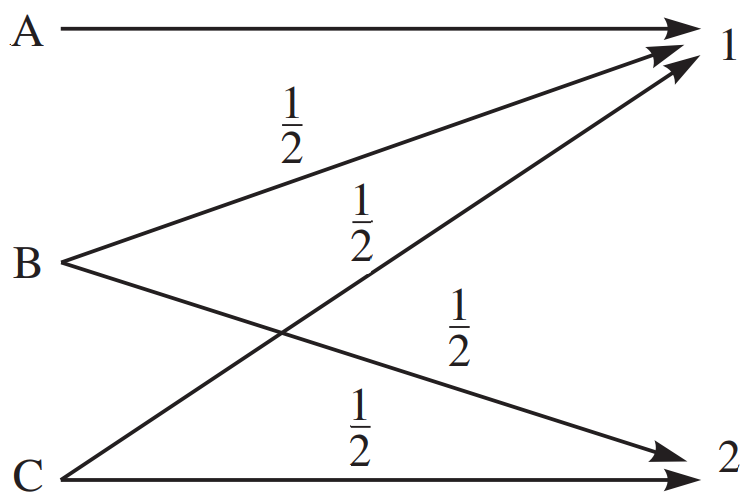
\includegraphics[scale=0.35]{Practice3-2-1.png}
                \caption{channel model}
                % \label{fig}
            \end{figure} \\ \\ 
            \textbf{Solution:} \\
            By symmetry of the inputs \textbf{B} and \textbf{C}, their probabilities have to be equal and we have 
            % $P(A) = 1 - p$, $P(B) = P(C) = p/2$. 
            \begin{align*}
                \begin{aligned}
                    \left\{
                    \begin{aligned}
                        & P(A) = 1 - p \\
                        & P(B) = P(C) = p/2
                    \end{aligned}
                    \right.
                \end{aligned}
            \end{align*}
            Then we have 
            \begin{align*}
                \begin{aligned}
                    \Rightarrow \;\; & \left\{
                    \begin{aligned}
                        & P(Y = 1) = 1 - p + p/2 = 1 - p/2 \\
                        & P(Y = 2) = p/2
                    \end{aligned}
                    \right. \\ 
                    \Rightarrow \;\; & \left\{
                    \begin{aligned}
                        & H_b(p) = -p \log_2 p - (1 - p) \log_2 (1 - p) \\
                        & H_b(\frac{p}{2}) = -\frac{p}{2} \log_2 \frac{p}{2} - (1 - \frac{p}{2}) \log_2 (1 - \frac{p}{2})
                    \end{aligned}
                    \right.
                \end{aligned}
            \end{align*}
            thus $H(Y) = H_b(p/2)$. We also note that 
            \begin{align*}
                \begin{aligned}
                    \left\{
                    \begin{aligned}
                        & H(Y|X = A) = 0 \\
                        & H(Y|X = B) = H(Y|X = C) = 1
                    \end{aligned}
                    \right.
                \end{aligned}
            \end{align*}
            hence 
            \begin{align*}
                & H(Y) = -\frac{p}{2} \log_2 \frac{p}{2} - (1 - \frac{p}{2}) \log_2 (1 - \frac{p}{2}) \\ 
                & H(Y|X) = (1 - p) \cdot H(Y|X = A) + p/2 \cdot H(Y|X = B)  + p/2 \cdot H(Y|X = C) = p
            \end{align*}
            Therefore, 
            \begin{align*}
                C &= \max_{p} I(X;Y) \\
                  &= \max_{p} H(Y) - H(Y|X) \\
                  &= \max_{p} H_b(p/2) - p \\ 
                  &= \max_{p} \left( -\frac{p}{2} \log_2 \frac{p}{2} - (1 - \frac{p}{2}) \log_2 (1 - \frac{p}{2}) \right) - p
            \end{align*}
            straightforward differentiation results in 
            \begin{align*}
                & \frac{dC}{dp} = \frac{d}{dp} \left( -\frac{p}{2} \log_2 \frac{p}{2} - (1 - \frac{p}{2}) \log_2 (1 - \frac{p}{2}) \right) - \frac{d}{dp} p = 0 \\ 
                \Rightarrow \; & - \left[ \frac{1}{2} \log_2 (\frac{p}{2}) + \frac{p}{2} \cdot \left( \frac{\frac{1}{2}}{\frac{p}{2} \ln 2} \right) - \frac{1}{2} \log_2 (1 - \frac{p}{2}) + (1 - \frac{p}{2}) \cdot \left( \frac{-\frac{1}{2}}{(1 - \frac{p}{2}) \ln 2}\right) \right] - 1 = 0 \\ 
                \Rightarrow \; & -\frac{1}{2} \log_2 (\frac{\frac{p}{2}}{1 - \frac{p}{2}} ) - 1 = 0 \;\;\; \left(\because \log_a b = \frac{\log_e b}{\log_e a} \right) \\
                \Rightarrow \; & -\frac{1}{2} \cdot \frac{\log_e (\frac{\frac{p}{2}}{1 - \frac{p}{2}})}{\log_e 2} - 1 = 0 \;\;\; \left(\because \log_a b = \frac{1}{\log_b a} \right) \\ 
                \Rightarrow \; & -\frac{1}{2} \log_2 e \cdot \ln (\frac{\frac{p}{2}}{1 - \frac{p}{2}}) - 1 = 0 \\
                % \Rightarrow \; & -\frac{1}{2} \log_2 e \ln (\frac{p/2}{1 - p/2}) - 1 = 0
                \Rightarrow \; & \ln (\frac{\frac{p}{2}}{1 - \frac{p}{2}}) = \frac{2}{\log_2 e} \;\;\;
                \Rightarrow \; \frac{\frac{p}{2}}{1 - \frac{p}{2}} = \exp(\frac{2}{\log_2 e}) = \frac{1}{4} \\ 
                \Rightarrow \; & \frac{p}{2} = \frac{1}{4} - \frac{p}{8} \;\;\; \Rightarrow \; \frac{5p}{8} = \frac{2}{8}
            \end{align*}
            resulting in 
            \begin{align*}
               p &= \frac{2}{5} = 0.4 \\ 
               C &= H_b(\frac{p}{2}) - p = \left(-\frac{p}{2} \log_2 \frac{p}{2} - (1 - \frac{p}{2}) \log_2 (1 - \frac{p}{2})\right) - p \\
                 &= H_b(0.2) - 0.4 = \left( -0.2 \log_2 0.2 - (1 - 0.2) \log_2 (1 - 0.2) \right) - 0.4 \\ 
                 &\approx 0.7219 - 0.4 = 0.3219
            \end{align*}
            \begin{flushright}
                $\blacksquare$
            \end{flushright}
    %%%%%%%%%%%%%%%%%%%%%%%%%%%%%%
        \item (12\%)
            % 3. (Practice #3 - 2, 9.14)
            A voice-band telephone channel passes the frequencies in the band from $300$ to $3300$ Hz. It is desired to design a modem that transmits at a symbol rate of $2400$ symbols/s, with the objective of achieving $9600$ bits/s. 
            \textbf{Select} an appropriate \textbf{QAM signal constellation}, \textbf{carrier frequency}, and the \textbf{roll-off factor} of a pulse with a raised cosine spectrum that utilizes the entire frequency band. 
            \textbf{Sketch the spectrum} of the transmitted signal pulse and \textbf{indicate the important frequencies}. \\ \\ 
            \textbf{Solution:} \\
            The bandwidth of the bandpass channel is:
            \begin{align*}
                W = 3300 - 300 = 3000 \; \text{Hz}
            \end{align*}
            In order to transmit $9600$ bps with a symbol rate
            \begin{align*}
                R = \frac{1}{T} = 2400 \;\; \text{symbols/sec}
            \end{align*}
            the number of information bits per symbol should be
            \begin{align*}
                k = \frac{9600}{2400} = 4 \; \text{bits}
            \end{align*}
            Hence, a $2^4 = 16$ QAM signal constellation is needed. \\ \\ 
            The carrier frequency $f_c$ is:
            \begin{align*}
                f_c = \frac{300 + 3300}{2} = 1800 \; \text{Hz}
            \end{align*}
            which is the mid-frequency of the frequency band that the bandpass channel occupies. If a pulse with raised cosine spectrum and roll-off factor $\beta$ is used for spectral shaping, then for the bandpass signal with bandwidth $W$:
            \begin{align*}
                & \frac{1}{2T}(1 + \beta) = \frac{W}{2} = 1500 \\
                & \Rightarrow \frac{1}{2} \cdot 2400 \cdot (1 + \beta) = 1500 \\
                & \Rightarrow 1 + \beta = \frac{1500}{1200} = 1.25 \\ 
                & \therefore \beta = 0.25
            \end{align*}
            \newpage
            A sketch of the spectrum of the transmitted signal pulse is shown in Figure 2. (The horizontal coordinate, say 3000, is computed as follows:
            $f_c + \frac{1}{2T} = 1800 + 2400 / 2 = 3000$)
            \begin{figure}[h]
            	\centering
            	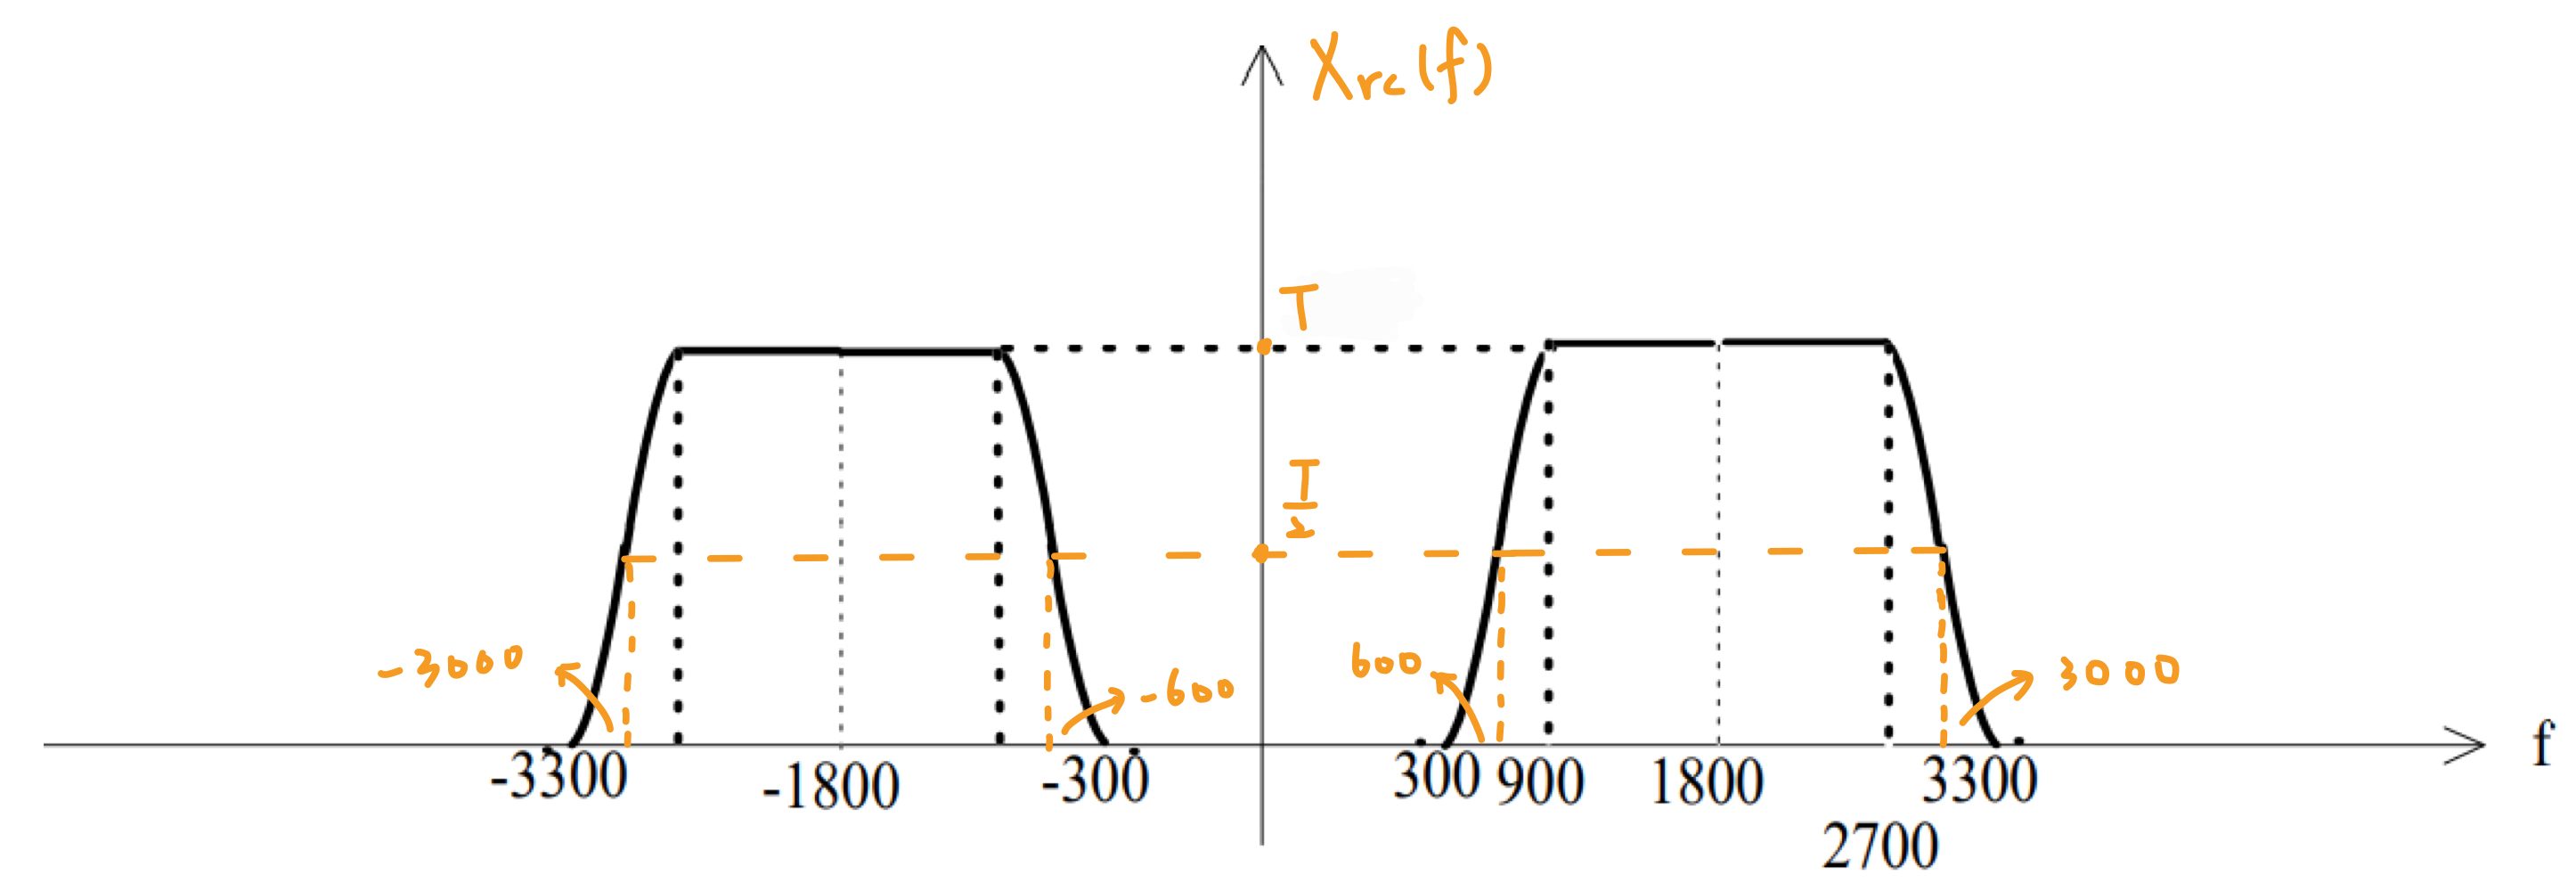
\includegraphics[scale=0.18]{Practice3-7-3.jpg}
            	\caption{transmitter block diagram}
            \end{figure}
            \begin{flushright}
                $\blacksquare$
            \end{flushright}
    %%%%%%%%%%%%%%%%%%%%%%%%%%%%%%  
        \item (24\%) 
            % 4. (4.24)
            Three equiprobable messages $m_1$, $m_2$ and $m_3$ are to be transmitted over an AWGN channel with noise power spectral density $\frac{1}{2}N_0$. The messages are 
            \begin{align*}
                s_1(t) = \left\{
                \begin{aligned}
                    & 1 \;\;\;\; 0 \leq t \leq T \\ 
                    & 0 \;\;\;\; \text{otherwise}
                \end{aligned}
                \right.
                \;\;\;\;\;\;
                s_2(t) = -s_3(t) \left\{
                \begin{aligned}
                     &1  \;\;\;\; 0 \leq t \leq \frac{1}{2}T \\ 
                    -&1 \;\;\;\; \frac{1}{2}T < t \leq T \\
                     &0  \;\;\;\; \text{otherwise}
                \end{aligned}
                \right.
            \end{align*}
            (a) What is the \textbf{dimensionality} of the signal space? \\ 
            (b) Find an \textbf{appropriate basis} for the signal space. \\ 
            (c) Please \textbf{Draw the signal constellation} of the messages $m_1$, $m_2$, $m_3$ and \textbf{the optimal decision regions} $R_1$, $R_2$, $R_3$ for this problem. \\ 
            (d) Which of the three messages is most vulnerable to errors and why? In other words, which of $P(\text{error} \ | \ m_i \; \text{transmitted}), \ i = 1, 2, 3$, is largest? \\ \\ 
            \textbf{Solution:} \\
            \textbf{(a)} Since $m_2(t) = -m_3(t)$ the dimensionality of the signal space is two. \\
            \textbf{(b)} As a basis of the signal space we consider the functions 
            \begin{align*}
                f_1(t) = \left\{
                \begin{aligned}
                    & \frac{1}{\sqrt{T}} \;\;\;\;  0 \leq t \leq T \\ 
                    & \;\;\; 0 \;\;\;\;\;\; \text{otherwise}
                \end{aligned}
                \right.
                \;\;\;
                f_2(t) = \left\{
                \begin{aligned}
                    &\frac{1}{\sqrt{T}}  \;\;\;\; 0 \leq t \leq \frac{1}{2}T \\ 
                    -&\frac{1}{\sqrt{T}} \;\;\;\; \frac{1}{2}T < t \leq T \\
                     & \;\;\; 0 \;\;\;\;\;\; \text{otherwise}
                \end{aligned}
                \right.
            \end{align*}
            The vector representation of the signals is 
            \begin{align*}
                \mathbf{m_1} = [\sqrt{T}, \ 0], \;\;\; \mathbf{m_2} = [0, \ \sqrt{T}], \;\;\; \mathbf{m_3} = [0, \ -\sqrt{T}]
            \end{align*}
            \newpage
            \textbf{(c)} The signal constellation and the decision regions is depicted in Figure 3.
            \begin{figure}[h]
                \centering
                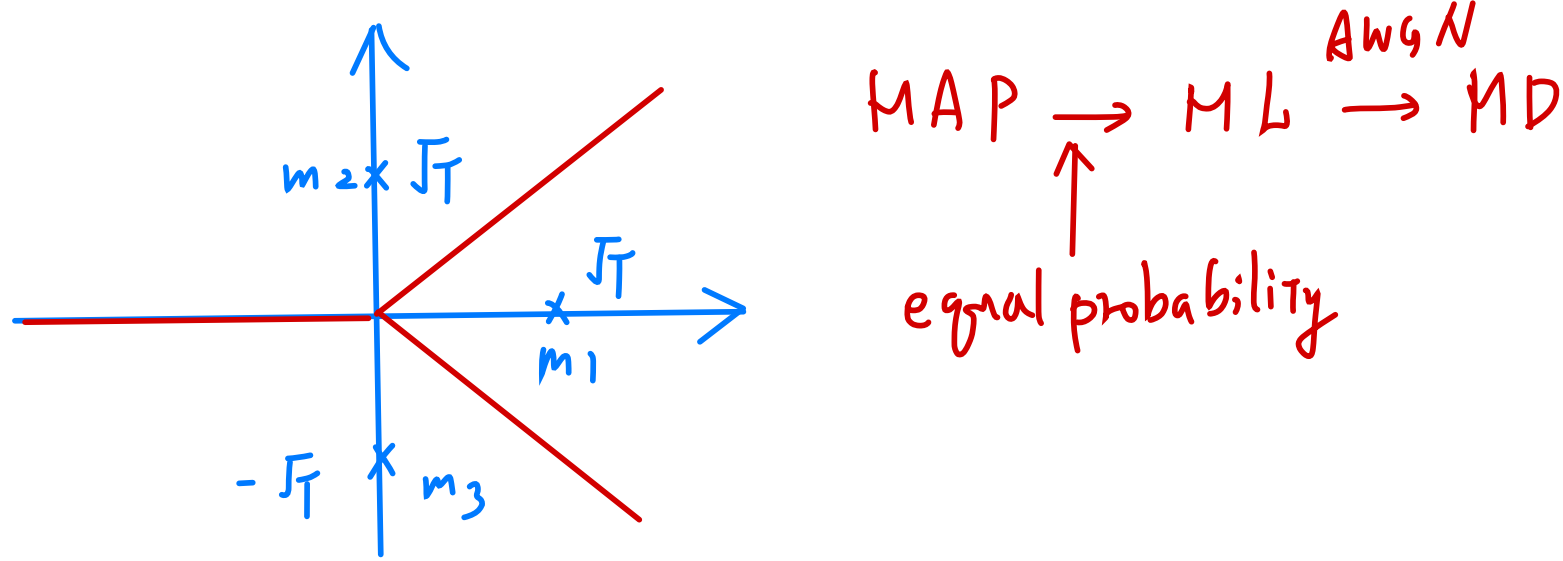
\includegraphics[scale=0.45]{Final-4-1.png}
                \caption{signal constellation and decision regions}
                % \label{fig:my_label}
            \end{figure} \\ 
            \textbf{(d)} If the signals are equiprobable then:
            \begin{align*}
                P(e | \bf{m_1}) = P(|r - m_1|^2 > |r - m_2|^2 | m_1) + P(|r - m_1|^2 > |r - m_3|^2 | m_1)
            \end{align*}
            When $\bf{m_1}$ is transmitted then $\bf{r} = \left[ \sqrt{T} + n_1, n_2 \right]$ and therefore, $P(e | \bf{m_1})$ is written as:
            \begin{align*}
                P(e | \bf{m_1}) = P(n_2 - n_1 > \sqrt{T}) + P(n_1 + n_2 < \sqrt{T})
            \end{align*}
            Since $n_1, n_2$ are zero-mean statistically independent Gaussian random variables, each with variance $\frac{N_0}{2}$, the random variables $x = n_1 - n_2$ and $y = n_1 + n_2$ are zero-mean Gaussian with variance $N_0$. 
            When $\bf{m_2}$ is transmitted then $\bf{r} = \left[n_1, n_2 + \sqrt{T}  \right]$ and therefore, $P(e | \bf{m_2})$ is written as:
            \begin{align*}
                P(e | \bf{m_2}) = P(n_1 - n_2 > \sqrt{T}) + P(n_2 < \sqrt{T})
            \end{align*}
            Similarly from the symmetry of the problem, we obtain:
            \begin{align*}
                P(e | \bf{m_3}) = P(e | \bf{m_2})
            \end{align*}
            Hence:
            \begin{align*}
                 % P_e(d_{\text{min}}) &= Q(\frac{d_{\text{min}}}{2\sigma}) = Q(\sqrt{\frac{(d_{\text{min}})^{2}}{2N_0}}) \\ 
                 P(e|\bf{m_1}) &= \frac{1}{\sqrt{2\pi N_0}} \int_{\sqrt{T}}^{\infty} e^{-\frac{x^2}{2N_0}} dx + \frac{1}{\sqrt{2\pi N_0}} \int_{-\infty}^{-\sqrt{T}} e^{-\frac{y^2}{2N_0}} dy \\ 
                          &= Q(\sqrt{\frac{2T}{2N_0}}) + Q(\sqrt{\frac{2T}{2N_0}}) = 2Q(\sqrt{\frac{T}{N_0}}) \\
                 P(e|\bf{m_2}) &= Q(\sqrt{\frac{2T}{2N_0}}) + Q(\sqrt{\frac{4T}{2N_0}}) = Q(\sqrt{\frac{T}{N_0}}) + Q(\sqrt{\frac{2T}{N_0}}) = P(e|\bf{m_3})
            \end{align*}
             Since $Q( \cdot )$  is momononically decreasing, we obtain: 
            \begin{align*}
                Q(\sqrt{\frac{2T}{N_0}}) < Q(\sqrt{\frac{T}{N_0}})
            \end{align*}
            and therefore, the probability of error $P(e|\bf{m_1})$ is larger than $P(e|\bf{m_2})$ and $P(e|\bf{m_3})$ Hence, the message $\bf{m_1}$ is more vulnerable to errors. The reason for that is that it has both threshold lines close to it, while the other two signals have one of the their threshold lines further away. 
            \newpage
            $\because \;$ The probability of error $P(e|\bf{m_1})$ is larger than $P(e|\bf{m_2})$ and $P(e|\bf{m_3})$. \\
            $\therefore \;$ The message $\bf{m_1}$ is the most vulnerable to errors.
            \begin{flushright}
                $\blacksquare$
            \end{flushright}
    %%%%%%%%%%%%%%%%%%%%%%%%%%%%%%  
        \item (24\%)
            % 5. (6.28)
            Two discrete memoryless information sources X and Y each have an alphabet with six symbols, $\mathcal{X} = \mathcal{Y} = \{ 1, 2, 3, 4, 5, 6 \}$. The probabilities of the letters for X are $\{ \frac{1}{2}$, $\frac{1}{4}$, $\frac{1}{8}$, $\frac{1}{16}$, $\frac{1}{32}$, $\frac{1}{32} \}$. The source Y has a uniform distribution. \\ 
            (a) Find the entropy of both X and Y. \\ 
            (b) Design Huffman codes for each source. Which Huffman code is more efficient? \\
            \textbf{(\textit{Hint}}: Efficiency of a Huffman code is defined as the ratio of the source entropy $H(X)$ to the average codeword length $\Bar{R}$.\textbf{)} \\
            (c) If Huffman codes were designed for the second extension of these sources (i.e., two letters at a time), \textbf{for which source (X or Y) would you expect a performance improvement} compared to the single-letter Huffman code and why? \\ \\
            \textbf{Solution:} \\ 
            \textbf{(a)} 
            % The entropy of X:
            \begin{align*}
                \text{The entropy of X:} \;\;\; 
                H(X) &= -\sum_{i = 1}^{5} (\frac{1}{2})^i \log_2 (\frac{1}{2})^i - \frac{1}{32} \log_2 \frac{1}{32} \\
                &= -\frac{1}{2} \log_2 \frac{1}{2} -\frac{1}{4} \log_2 \frac{1}{4} -\frac{1}{8} \log_2 \frac{1}{8} -\frac{1}{16} \log_2 \frac{1}{16} -\frac{2}{32} \log_2 \frac{1}{32} \\
                &= \frac{1}{2} \log_2 2 + \frac{1}{4} \log_2 4 + \frac{1}{8} \log_2 8 + \frac{1}{16} \log_2 16 + \frac{1}{16} \log_2 32 \\ 
                &= \frac{1}{2} \cdot 1 + \frac{1}{4} \cdot 2 + \frac{1}{8} \cdot 3 + \frac{1}{16} \cdot 4 + \frac{1}{16} \cdot 5 \\ 
                &= \frac{8}{16} + \frac{8}{16} + \frac{6}{16} + \frac{4}{16} + \frac{5}{16} = \frac{31}{16} = 1.9375 \\ 
                \text{The entropy of Y:} \;\;\; H(Y) &= 6 \cdot (- \frac{1}{6} \log_2 \frac{1}{6}) = \log_2 6 = 2.5850
            \end{align*}
            % The entropy of Y:
            % \begin{align*}
            %     H(Y) &= 6 \cdot (- \frac{1}{6} \log_2 \frac{1}{6}) = \log_2 6 = 2.5850
            % \end{align*}
            \textbf{(b)} For X the Huffman tree is
            \begin{figure}[h]
                \centering
                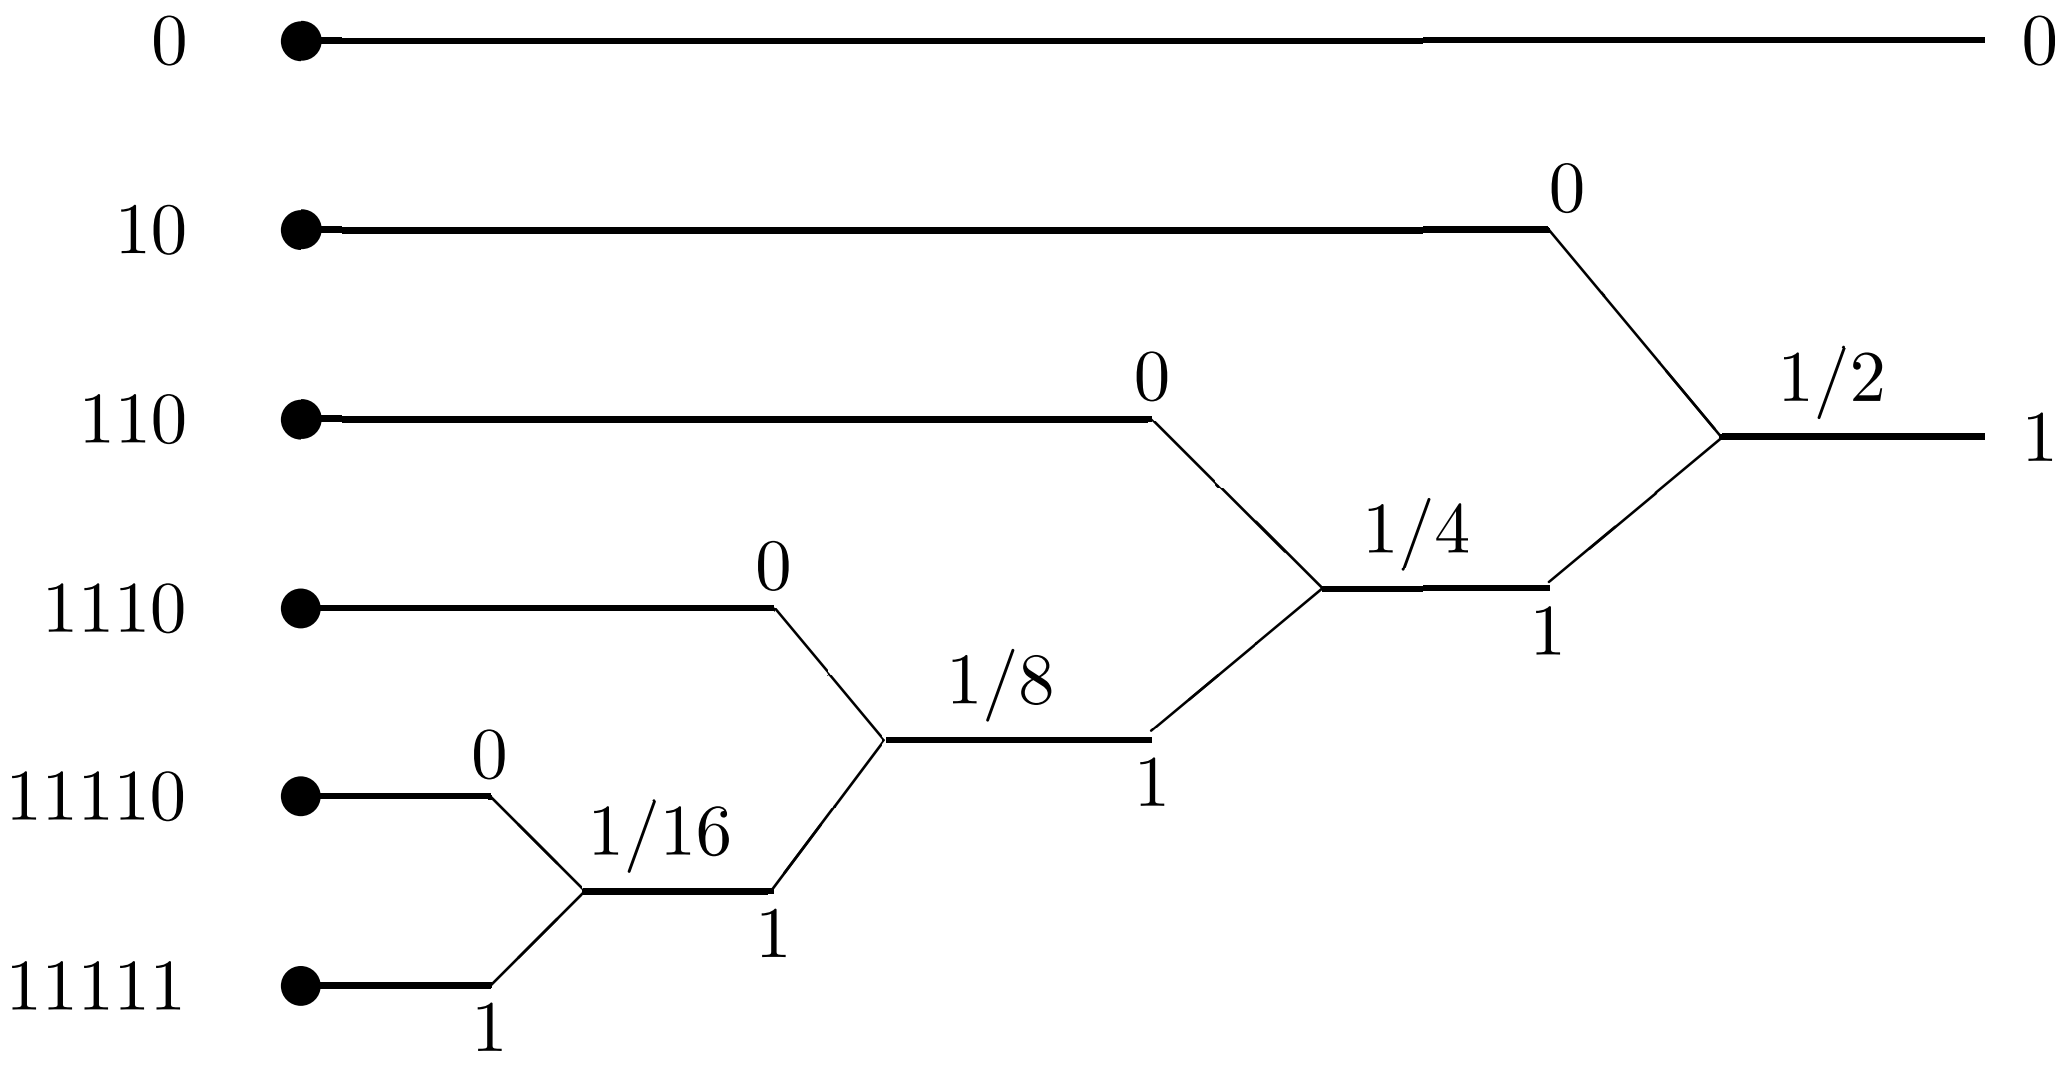
\includegraphics[scale=0.25]{Final-5-x_tree.png}
                \caption{the Huffman tree of X}
                % \label{fig:my_label}
            \end{figure}
            \newpage
            and for Y the Huffman tree is
            \begin{figure}[h]
                \centering
                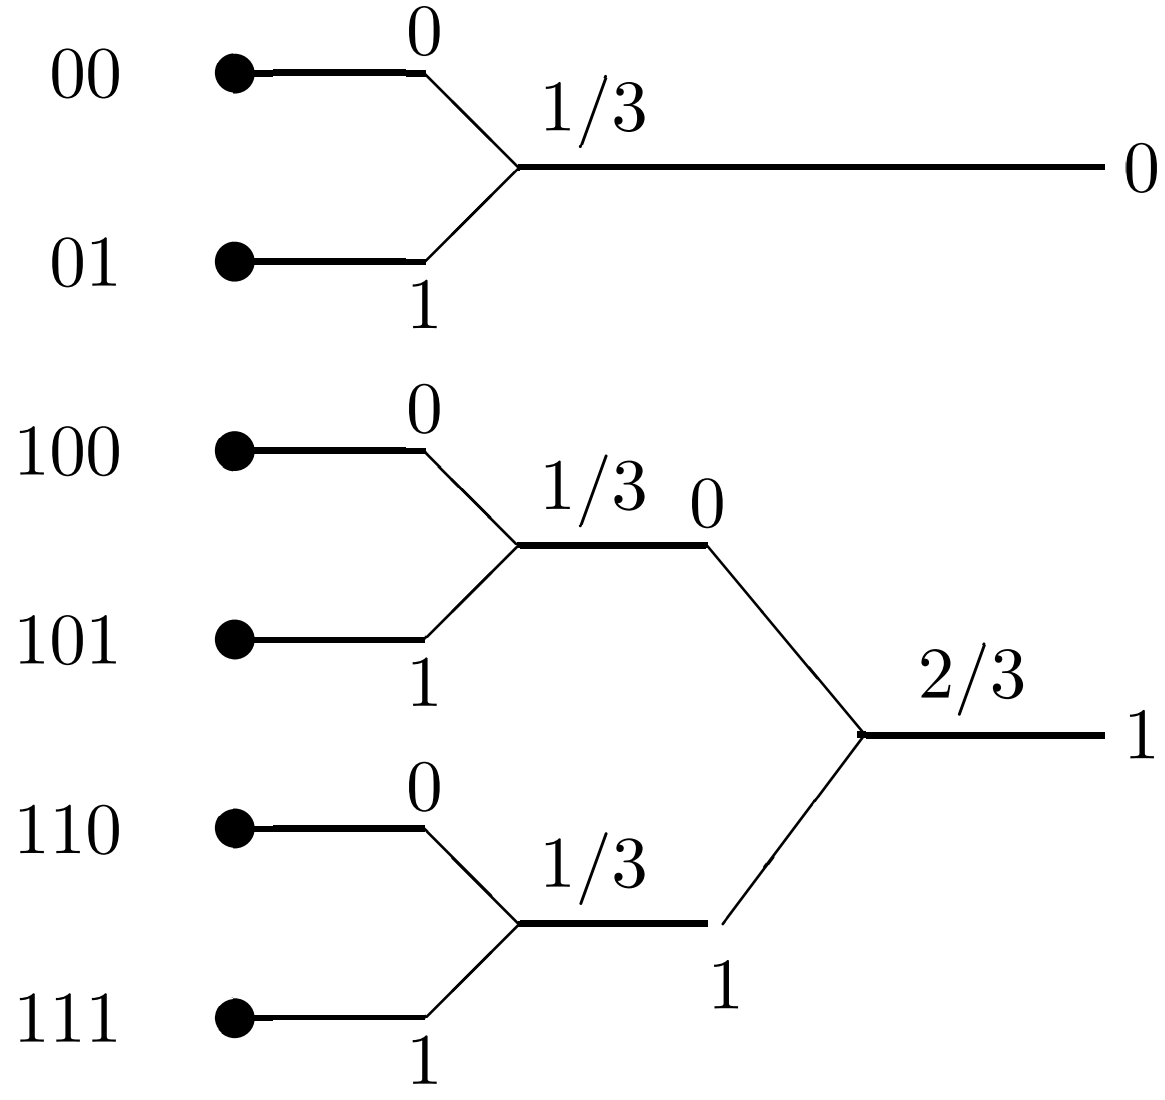
\includegraphics[scale=0.25]{Final-5-y_tree.png}
                \caption{the Huffman tree of Y}
                % \label{fig:my_label}
            \end{figure} \\ 
            For X the average codeword length is
            \begin{align*}
                \Bar{R}_X &= 1 \cdot \frac{1}{2} + 2 \cdot \frac{1}{4} + 3 \cdot \frac{1}{8} + 4 \cdot \frac{1}{16} + 5 \cdot \frac{2}{32} \\
                        &= \frac{8}{16} + \frac{8}{16} + \frac{6}{16} + \frac{4}{16} + \frac{5}{16} = \frac{31}{16} = 1.9375
            \end{align*}
            hence the efficiency of X is
            \begin{align*}
                \eta_{X} = \frac{H(X)}{\Bar{R}_X} = \frac{1.9375}{1.9375} = 1 = 100 \%
            \end{align*}
            For Y the average codeword length is
            \begin{align*}
                \Bar{R}_Y &= 2 \cdot \frac{1}{3} + 3 \cdot \frac{2}{3} = \frac{8}{3} = 2.666
            \end{align*}
            hence the efficiency of Y is
            \begin{align*}
                \eta_{Y} = \frac{H(Y)}{\Bar{R}_Y} = \frac{2.5850}{2.666} \approx 0.9696 = 96.96 \%
            \end{align*}
            Therefore X is more efficient. \\ \\ 
            \textbf{(c)} Source X has achieved 100\% efficiency. Therefore we expect an improvement for source Y.
            \begin{flushright}
                $\blacksquare$
            \end{flushright}
    %%%%%%%%%%%%%%%%%%%%%%%%%%%%%%    
        \item (16\%)
            % 6. (9.42 + 9.41 ZF)
            The transmission of a signal pulse with a raised cosine spectrum through a channel results in the following \textbf{(noise-free)} sampled output from the demodulator: 
            \begin{align*}
                x_k = \left\{
                \begin{aligned}
                    -0.&5 \;\;\; m = -2 \\ 
                     0.&1 \;\;\; m = -1 \\ 
                       &1 \;\;\; m = 0 \\ 
                    -0.&2 \;\;\; m = 1 \\ 
                    0.0&5 \;\;\; m = 2 \\ 
                       &0 \;\;\; \text{otherwise} \\ 
                \end{aligned}
                \right.
            \end{align*}
            (a) Design a three-tap zero-forcing linear equalizer so that the output is 
            \begin{align*}
                q_m = \left\{
                \begin{aligned}
                    & 1 \;\;\; m = 0 \\ 
                    & 0 \;\;\; m = \pm 1 
                \end{aligned}
                \right.
            \end{align*}
            (b) Determine $q_m$ for $m = \pm 2, \pm 3$ by convolving the impulse response of the equalizer with the channel response. \\ \\ 
            \textbf{Solution:} \\
            \textbf{(a)} The output of the zero-forcing linear equalizer is:
            \begin{align*}
                & q_m = \sum_{n = -1}^{1} c_n x_{m - n} \\ 
                \Rightarrow \;\; & \left\{
                \begin{aligned}
                    & x_{0}c_{-1} + x_{-1}c_{0} + x_{-2}c_{1} = q_{-1} \\
                    & x_{1}c_{-1} + x_{0}c_{0} + x_{-1}c_{1} = q_{0} \\ 
                    & x_{2}c_{-1} + x_{1}c_{0} + x_{0}c_{1} = q_{1} 
                \end{aligned}
                \right. \;\;
                \Rightarrow \;\; \left(
                \begin{array}{c c c}
                    x_{0} &  x_{-1} & x_{-2} \\ 
                    x_{1} &  x_{0} & x_{-1} \\
                    x_{2} & x_{1} & x_{0} 
                \end{array}
                \right)
                \left(
                \begin{array}{c}
                    c_{-1} \\ 
                    c_0 \\
                    c_1  
                \end{array}
                \right)
                = \left(
                \begin{array}{c}
                    q_{-1} \\ 
                    q_{0} \\
                    q_{1}  
                \end{array}
                \right)
                % \Rightarrow \;\; & x_{0}c_{-1} + x_{-1}c_{0} + x_{-2}c_{1} = q_{-1} \\ 
                % \Rightarrow \;\; & x_{1}c_{-1} + x_{0}c_{0} + x_{-1}c_{1} = q_{0} \\ 
                % \Rightarrow \;\; & x_{2}c_{-1} + x_{1}c_{0} + x_{0}c_{1} = q_{1} 
            \end{align*}
            With $q_0 = 1$ and $q_1 = 0$ for $m \neq 0$, we obtain the system:
            \begin{align*}
                \left(
                \begin{array}{c c c}
                     1 &  0.1 & -0.5 \\ 
                    -0.2 &  1 & 0.1 \\
                    0.05 & -0.2 & 1 
                \end{array}
                \right)
                \left(
                \begin{array}{c}
                    c_{-1} \\ 
                    c_0 \\
                    c_1  
                \end{array}
                \right)
                = \left(
                \begin{array}{c}
                    0 \\ 
                    1 \\
                    0  
                \end{array}
                \right)
            \end{align*}
            Solving the previous system in terms of the equalizer's coefficients, we obtain:
            \begin{align*}
                \left(
                \begin{array}{c}
                    c_{-1} \\ 
                    c_0 \\
                    c_1  
                \end{array}
                \right)
                &= \left(
                \begin{array}{c c c}
                     1 &  0.1 & -0.5 \\ 
                    -0.2 &  1 & 0.1 \\
                    0.05 & -0.2 & 1 
                \end{array}
                \right)^{-1}
                \left(
                \begin{array}{c}
                    0 \\ 
                    1 \\
                    0  
                \end{array}
                \right) \\ 
                &\approx \left(
                \begin{array}{c c c}
                    0.9756 & 0 & 0.4878 \\ 
                    0.1961 & 0.9804 & 0 \\ 
                    0.0096 & 0.1961 & 0.9756
                    % \frac{40}{41} &  0 & \frac{20}{41} \\ 
                    % \frac{10}{51} &  \frac{50}{51} & 0 \\
                    % \frac{-20}{2091} & \frac{10}{51} & \frac{40}{41} 
                    % 40/41	      0	    20/41
                    % 10/51	    50/51	  0
                    % -20/2091	10/51	40/41
                \end{array}
                \right)
                \left(
                \begin{array}{c}
                    0 \\ 
                    1 \\
                    0 
                \end{array}
                \right)
                =\left(
            \begin{array}{c}
                0 \\ 
                0.9804 \\ % 0.980392
                0.1961  % 0.196078
            \end{array}
            \right)
            \end{align*}
            \textbf{(b)} The output values of the equalizer $q_m$ for $m = \pm 2, \pm 3$ are given by 
            % c_{}x_{}
            \begin{align*}
                q_{-3} &=  \sum_{n = -1}^{1} c_n x_{-3 - n} = c_{-1}x_{-2} + c_{0}x_{-3} + c_{1}x_{-4} = 0 + 0 + 0 = 0 \\ 
                q_{-2} &=  \sum_{n = -1}^{1} c_n x_{-2 - n} = c_{-1}x_{-1} + c_{0}x_{-2} + c_{1}x_{-3} = 0 + 0.9804 \cdot (-0.5) + 0 = -0.490196 \\
                q_2 &= \sum_{n = -1}^{1} c_n x_{2 - n} = c_{-1}x_{3} + c_{0}x_{2} + c_{1}x_{1} = 0 + 0.9804 \cdot 0.05 + 0.1961 \cdot (-0.2) = 0.0098 \\ 
                q_3 &= \sum_{n = -1}^{1} c_n x_{3 - n} = c_{-1}x_{4} + c_{0}x_{3} + c_{1}x_{2} = 0 + 0 + 0.1961 \cdot 0.05 = 0.009805
            \end{align*}
            Therefore
            \begin{align*}
                q_m = \left\{
                \begin{aligned}
                     &0 && m = -3 \\ 
                    -&0.490196 && m = -2 \\ 
                     &0.0098 && m = 2 \\ 
                     &0.009805 && m = 3
                \end{aligned}
                \right.
            \end{align*}
            \begin{flushright}
                $\blacksquare$
            \end{flushright} 
    %%%%%%%%%%%%%%%%%%%%%%%%%%%%%%
    \end{enumerate}
    \rule{\textwidth}{0.4pt}
\end{document}

